\documentclass{article}
\usepackage[utf8]{inputenc}
\usepackage{geometry}
\usepackage{graphicx}
\geometry{a4paper, margin=1in}

\title{Dokumentace k semestrální práci KIV/UPS Server-Klient Blackjack}
\author{Jan Vandlíček}
\date{\today}

\begin{document}

\maketitle

\section{Základní popis hry blackjack}
Projekt implementuje klasickou hru Blackjack, ve které hráči snaží dosáhnout součtu hodnot karet blížícího se 21, aniž by překročili tuto hodnotu. Server spravuje hru a komunikuje s klienty, kteří představují hráče. Hra je implementována bez dealera a eso má hodnotu "1".

\section{Popis protokolu}
\subsection{Formát zpráv}
Zprávy jsou formátovány jako textové řetězce s předem definovanými příkazy a parametry. Každá zpráva začíná hesle, následovaným příkazem adaty specifickými pro daný příkaz.

\subsection{Možné zprávy}

\begin{itemize}
    \item \textbf{NICK}: Příkaz pro nastavení přezdívky (nickname).
    \item \textbf{PING}: Příkaz pro odeslání ping zprávy.
    \item \textbf{PONG}: Příkaz pro odpověď na ping zprávu.
    \item \textbf{JOIN}: Příkaz pro připojení k serveru/hře.
    \item \textbf{PLAY}: Příkaz pro spuštění hry.
    \item \textbf{GMIF}: Příkaz pro získání informací o hrách.
    \item \textbf{GMJN}: Příkaz pro připojení k hře.
    \item \textbf{GMCK}: Příkaz pro ověření, zda může začít hra.
    \item \textbf{GMST}: Příkaz pro spuštění hry.
    \item \textbf{GMEN}: Příkaz pro ukončení hry.
    \item \textbf{TURN}: Příkaz pro provedení tahu v hře.
    \item \textbf{NEXT}: Příkaz pro zahájení dalšího kola hry.
    \item \textbf{STOP}: Příkaz pro zastavení akce nebo procesu.
    \item \textbf{RETR}: Příkaz pro získání stavu hry.
    \item \textbf{STAT}: Příkaz pro nastavení stavu.
    \item \textbf{KILL}: Příkaz pro ukončení nebo zastavení něčeho.
    \item \textbf{KIL2}: Další variace příkazu pro ukončení nebo zastavení něčeho.
\end{itemize}

\subsection{Přenášené struktury a datové typy}
Struktury zahrnují \texttt{Player}, \texttt{Game}, \texttt{Hand}, \texttt{Card} a další. Datové typy zahrnují celá čísla, řetězce a seznamy.

\subsection{Význam a kódy přenášených dat}
Každý datový prvek má specifický význam, například \texttt{Player} obsahuje informace o hráči, \texttt{Game} o stavech hry.

\subsection{Omezení a validace dat}
Data jsou validována pro integritu a platnost, například hodnoty karet nesmí překročit určité meze.

\subsection{Stavový diagram}
Diagram by zobrazil postupnou výměnu zpráv mezi klientem a serverem pro různé fáze hry.

\begin{figure}[htbp] % Specifikuje umístění obrázku (h - here, t - top, b - bottom, p - separate page)
    \centering % Zarovná obrázek na střed
    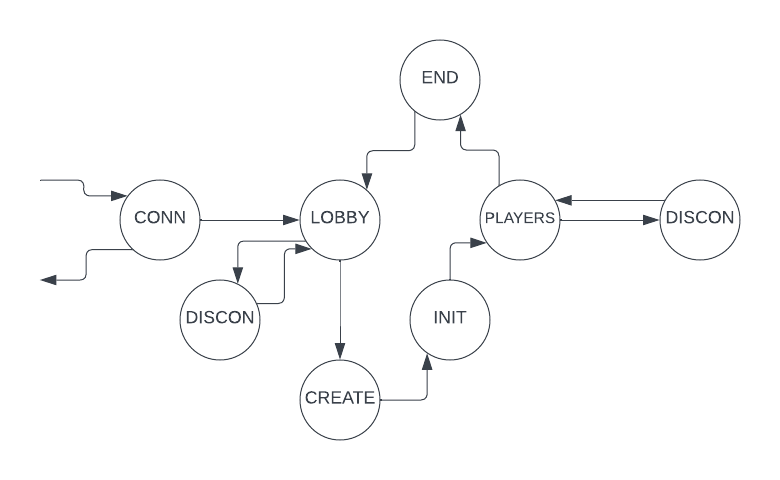
\includegraphics[width=0.6\textwidth]{img/diagram.png} % Specifikuje název a relativní šířku obrázku
    \caption{Stavový diagram pro hru Blakcjack} % Popisek nebo titulek obrázku
    \label{fig:obrazek} % Identifikátor pro odkazování na obrázek
\end{figure}

\subsection{Chybové stavy}
Chybové stavy zahrnují problémy s připojením, neplatné zprávy apod. Každá chyba má specifický kód a popis.

\section{Popis implementace klienta a serveru}
\subsection{Dekompozice do Modulů/Tříd}
Server i klient jsou rozděleni do několika modulů, každý s vlastní funkcionalitou.

\subsubsection{Server (Go)}
\begin{itemize}
  \item \textbf{server.go}: Hlavní modul serveru, zodpovědný za inicializaci hry, správu herních místností a zpracování připojení klientů.
  \item \textbf{game.go, player.go, hand.go, deck.go, card.go}: Tyto moduly definují základní struktury hry, včetně hráčů, karet, balíčků a herních rukou.
  \item \textbf{table\_status.go}: Obsahuje strukturu pro udržení stavu herního stolu.
  \item \textbf{comm.go, communication.go}: Zabývají se komunikací a zasíláním zpráv mezi serverem a klienty.
\end{itemize}

\subsubsection{Klient (Python)}
\begin{itemize}
  \item \textbf{main.py}: Hlavní spouštěcí bod aplikace klienta, zahajuje uživatelské rozhraní a zpracovává události.
  \item \textbf{client\_to\_server\_message.py}: Obsahuje funkce pro tvorbu a zpracování zpráv odesílaných serveru.
  \item \textbf{validation.py}: Zajišťuje validaci vstupních dat a zobrazuje upozornění.
  \item \textbf{msg\_const.py}: Definuje konstanty a parametry pro zprávy používané v komunikaci s serverem.
\end{itemize}

\subsection{Rozvrstvení aplikace}
Server a klient jsou strukturováni do vrstev, zahrnujících síťovou komunikaci, logiku hry a uživatelské rozhraní.

\subsubsection{Server (Go)}
\begin{itemize}
  \item \textbf{Síťová Vrstva}: Zpracovává síťové požadavky a komunikuje s klienty.
  \item \textbf{Logická Vrstva}: Obsahuje herní logiku a pravidla Blackjacku.
  \item \textbf{Datová Vrstva}: Ukládá a spravuje stav hry, hráče a herní objekty.
\end{itemize}

\subsubsection{Klient (Python)}
\begin{itemize}
  \item \textbf{Grafické Uživatelské Rozhraní (GUI)}: Umožňuje hráči interakci s hrou prostřednictvím grafického rozhraní.
  \item \textbf{Komunikační Modul}: Zajišťuje komunikaci s herním serverem.
  \item \textbf{Logická Vrstva}: Zpracovává herní logiku na straně klienta, jako jsou herní rozhodnutí a akce hráče.
\end{itemize}

\subsection{Použité knihovny a verze prostředí}
Využívá se GO 1.21 pro server a Python 3.9.2 spolu s knihvnou Tkinter pro klienta.

\subsection{Metoda paralelizace}
Server využívá gorutiny pro paralelní zpracování požadavků klientů.

\subsubsection{Server (Go)}
\begin{itemize}
  \item Využívá \textbf{gorutiny} pro asynchronní a paralelní zpracování. Například, server může současně spravovat více herních místností a klientů, každý běžící v samostatné gorutině.
  \item \textbf{Synchronizace}: Pro zajištění bezpečnosti při přístupu k sdíleným zdrojům používá mutexy a další synchronizační mechanismy.
\end{itemize}

\subsubsection{Klient (Python)}
\begin{itemize}
  \item Ačkoliv konkrétní metody paralelizace nejsou v poskytnutých souborech explicitně uvedeny, v GUI aplikacích běžně dochází k asynchronnímu zpracování událostí. 
  \item Může využívat vlákna nebo asynchronní funkce pro zpracování komunikace s serverem, zatímco GUI zůstává reaktivní.
\end{itemize}

\section{Požadavky na překlad, spuštění a běh aplikace}
\subsection{Verze jazyků a nástrojů}

\subsubsection{Server - GO}

Aplikace pro Server byla napsána v jazyce GO, konkrétně ve verzi 1.21.

\subsubsection{Klient - Python}

Aplikeace pro Klient byla napsána v jazyce Python , konkrétně ve verzi 3.9.2. Pro klient, respektive jeho GUI byla použita knihovna Tkiner.

\subsection{Postup překladu}

\subsubsection{Server - GO}

Pro spuštění serveru je třeba mít nainstalovanou správnou verzi jazyka GO (1.21), otevřít adresář, kde se nechází hlavní soubor \texttt{server.go} a spustit ho pomocí příkazu \texttt{go run server.go} v příkazové řádce.

Program serveru byl napsán pro operační systém Linux.

\subsubsection{Klient - Python}

Pro spuštění klienta je třeba mít nainstalovanou správnou verzi jazyka Python (3.9.2), otevřít adresář, kde se nechází hlavní soubor \texttt{main.py} a spustit ho pomocí příkazu \texttt{python3 main.py} v příkazové řádce.

Program klienta byl napsán pro operační systém Linux a Windows.

Pokud je třeba doinstalovat knihovnu Tkiner. Je to možno provést pomocí příkazu \texttt{pip install Tk}.

\section{Závěr}
Semestrální práce byla vyvíjena v domácím prostředí a následně testována na školních zařízeních pro její správné odevzdání, tento proces trochu práci zkomplikoval, ale byla mi tak předána zkušenost s vývojem aplikace pro různá zařízení. Výsledná aplikace je funčkní jak na zařízeních v domácí síti, tak na zařízeních školních. Je možno zahrát se ve více lidech karetní hru blackjack s opakováním a s vlastnostmi krátkodobého a dlouhodobého odpojení.

\end{document}